\documentclass{article}
\usepackage{pgfplots}
\pgfplotsset{compat=1.18}

\begin{document}

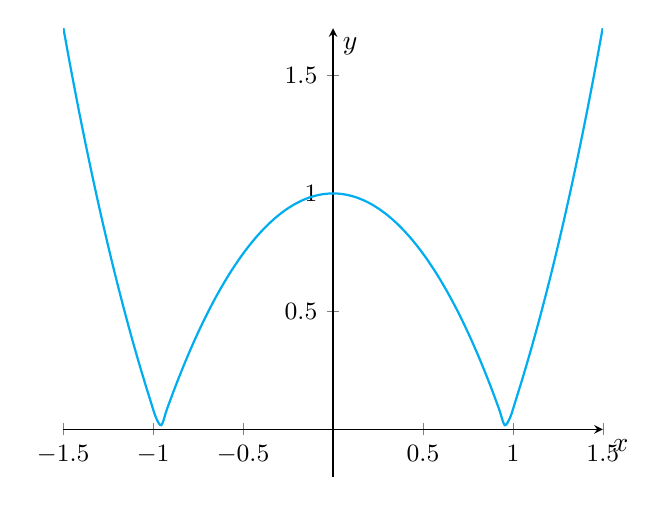
\begin{tikzpicture}
    \begin{axis}[
        axis lines = center,
        xlabel = {$x$},
        ylabel = {$y$},
        ymin=-0.2, ymax=1.7,
        xmin=-1.5, xmax=1.5,
        domain=-1.5:1.5,
        samples=100,
        smooth,
        ticklabel style={font=\small},
        label style={anchor=north west},
        every axis plot post/.append style={
            thick,
            color=cyan
        }
    ]
        \addplot [no markers] {abs(exp(x) + exp(-x) - 3)};
    \end{axis}
\end{tikzpicture}

\captionof{figure}{$f(x) = |e^x + e^{-x} - 3|$ exhibits exponential growth as $\|x\| \rightarrow + \infty$}

\end{document}